% SPDX-FileCopyrightText: Copyright (c) 2020-2025 Yegor Bugayenko
% SPDX-License-Identifier: MIT

\documentclass{article}
\usepackage{geometry}

\geometry{paperwidth=300pt, paperheight=250pt, left=10pt, right=10pt, top=10pt, bottom=10pt}

\usepackage[absolute]{textpos}\TPGrid{16}{16}
\usepackage{fancyhdr}
  \pagestyle{fancy}
  \renewcommand{\headrulewidth}{0pt}
  \fancyhf{}
\usepackage{graphicx}
\usepackage{bold-extra}
\usepackage{anyfontsize}
\usepackage{xcolor}
  \definecolor{xblack}{HTML}{1a1919}
  \definecolor{xred}{HTML}{b22222}
\begin{document}
\fontfamily{cmtt}\selectfont
\raggedbottom
\raggedright
\setlength{\topskip}{6pt}
\setlength{\parindent}{0pt} % indent first line
\setlength{\parskip}{6pt} % before par
\color{xblack}

\newcommand\invert[1]{\colorbox{xred}{\textcolor{white}{#1}}}

\begin{textblock}{14}[1,1](15,31)
  \raggedleft
  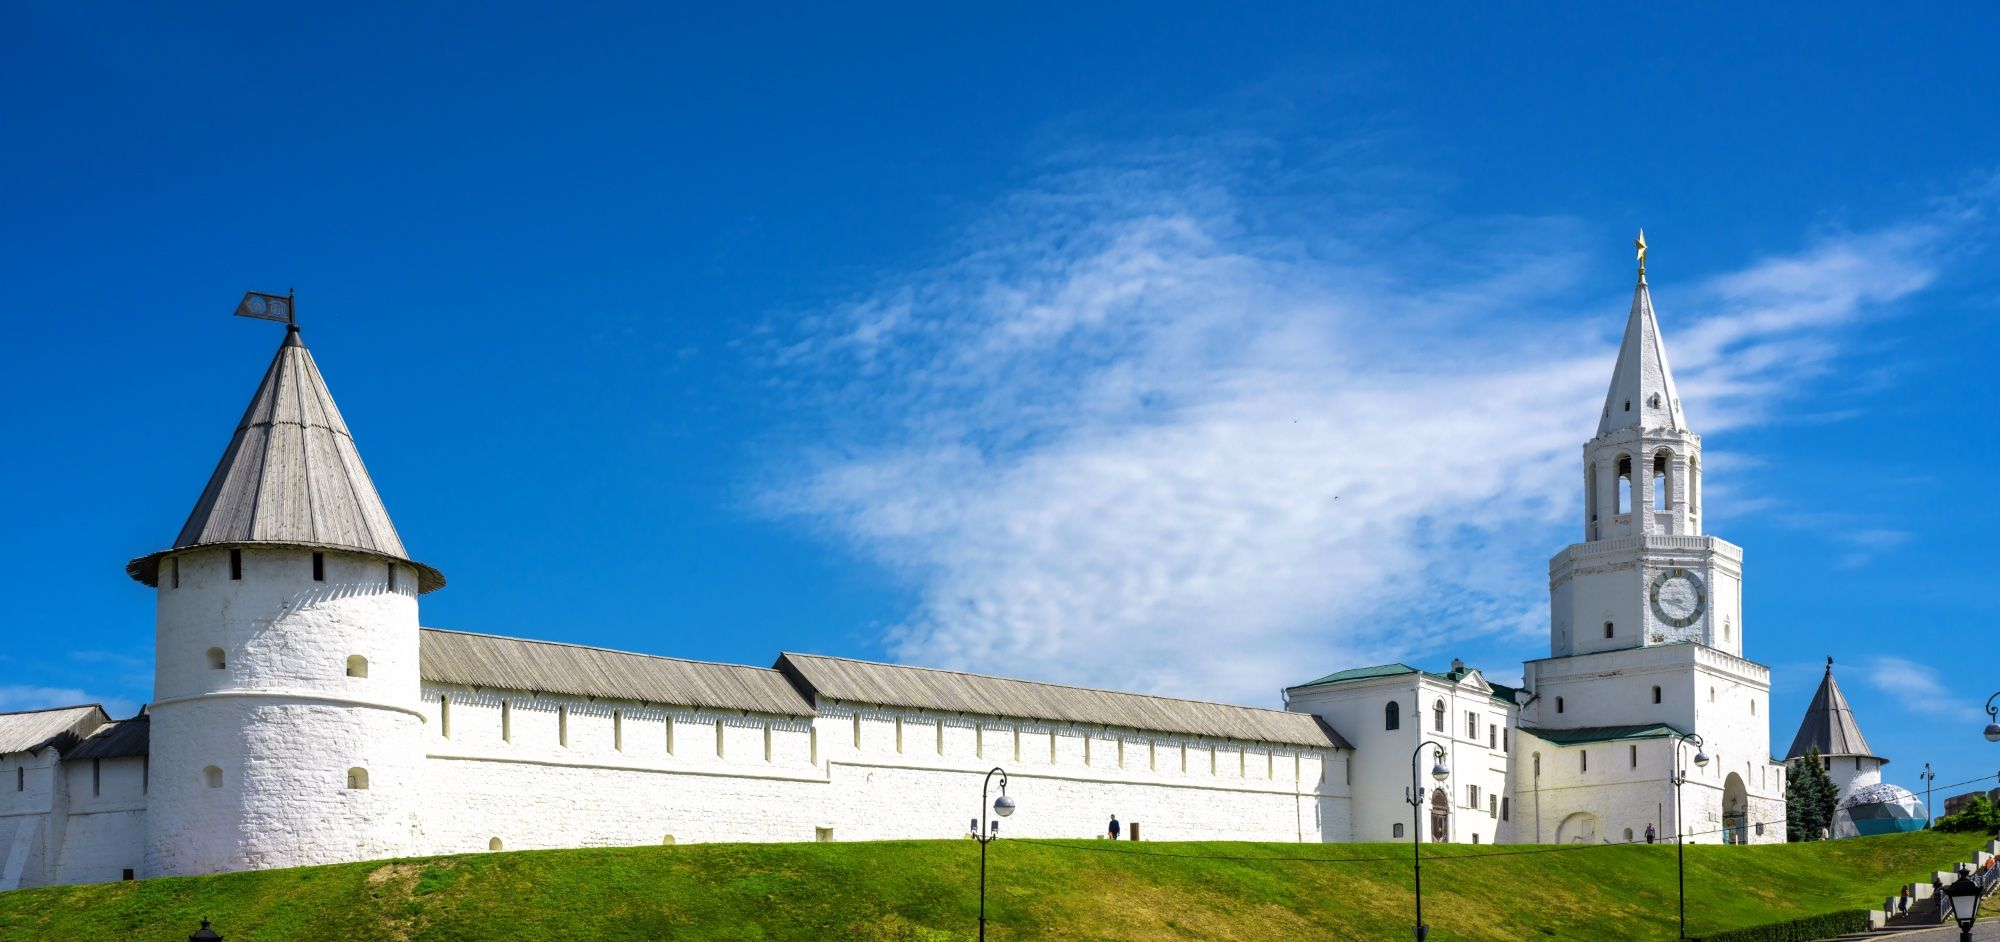
\includegraphics[width=14\TPHorizModule]{../../cfp/kazan}
\end{textblock}

\invert{\fontsize{64}{64}\selectfont\bfseries ICCQ}\\[24pt]
{\fontsize{18}{18}\selectfont\bfseries\color{xred}CfP: \\ \invert{18 Feb} \\}

\begin{textblock}{10}[1,1](15,15)
\fontsize{16}{16}\selectfont\bfseries
\raggedleft
The 4th \\
International \\
Conference \\
on \invert{Code Quality}

\vspace*{12pt}
In cooperation with \\
IEEE Computer Society

\vspace*{12pt}
Bug Detection \\
Program Analysis \\
Software Maintenance
\end{textblock}

\end{document}
